\documentclass{article}
\usepackage{graphicx}
\usepackage[a4paper, total={6in, 9in}]{geometry}
\usepackage[style=alphabetic,sorting=ynt]{biblatex}
\addbibresource{biblio.bib}

\begin{document}

\title{On the relation of spectral sampling and RV accuracy in echelle spectrographs}
\author{Marcelo Tala Pinto, Rafael Brahm, Leonardo Vanzi}

\maketitle


\section{Introduction}
Detectors with pixels on a square array are in widespread use in current optical and IR spectrographs. A key issue in the design of such instruments is the size of the individual detector pixels with respect to the width of the instrumental profile - in other words how many pixels should be used to sample the width of an unresolved spectral line. If too few pixels are used, narrow or unresolved spectral features will be undersampled, resulting in errors of position (i.e. wavelength) and possibly also flux which vary depending on the phase of the spectral line with respect to the pixel centers. This source of uncertainty becomes extremely relevant in exoplanet searches when trying to measure precision stellar radial velocities (RVs) using echelle spectrographs, as the typical RV shift produced by an orbiting planet is of the order of 1/1000 of a pixel. {\bf On the other side if too many pixels etc .... so that a suiitable pixel economy turns to be a critical aspect in the design of a spectrograph.}

The main goal of this document {\bf (paper?)} is to study theoretically the effect of detector pixelization in the measurement of stellar radial velocities (RV) using echelle spectrographs. {\bf Let's make it as general as possible. We used the optical design of PLATOSpec (REF), which is a pretty standard white pupile echelle, as test bench for the study. This will allow us to quantify the suitability of a given detector for the PLATOSPEC spectrograph.} 

{\bf First the simple and very general aproach by Rafael. Then... } We performed a series of stellar spectra simulations using the ray tracing software $\texttt{moes}$. This modeling scheme is based on direct ray tracing of the chief ray from the slit to the detector plane of an echelle spectrograph, applying exact corrections when tracing through curved surfaces \cite{moes}. The direct ray tracing provides an accurate theoretical description of the instrument as it calculates the exact the position of each ray along the optical path of the spectrograph.

Based on a synthetic spectrum of a G-type star, we created a series of spectra observations for a grid of RV shifts and detectors. Then we calculate the cross-correlation function (CCF, \cite{Queloz95}) to the simulated spectra to measure their RV. By comparing the nominal RV shift given to the spectra and the one measured using the CCF we can quantify the RV accuracy of the instrument. We calculate the RV accuracy of the instrument for a series of detectors that have the same size (27.6mm$\times$27.6mm) but different number of pixels and pixel sizes. By doing this it is possible to study the relation between pixelization of the spectra and the RV accuracy of the instrument.

\section{MOES PLATOSPEC}
PLATOSpec will be a state-of-the art echelle spectrograph with an average spectral resolution of 70\,000, covering the spectral range from 350nm to 700nm, which will be dedicated to ground-based support of space missions TESS, PLATO and later ARIEL. PLATOSpec is designed to achieve accuracy in radial velocities down to 5 m/s with using of simultaneous ThAr and optionally Iodine cell calibrations. {\bf here you need to refere basically to Angelica's paper}

The instrument is currently in the design phase, hence we have used the preliminary optical design to build the $\texttt{moes}$ ray tracing model for PLATOSPEC. The instrument modeled consist of: a slit, a two parabolic mirror collimators (C1 and C2), an echelle grating as the main dispersing element (EG), a flat transfer mirror (TM), a transmission grating as a cross-dispersing element (CG), a paraxial camera (PC) and a detector (CCD). Fig.~\ref{fig:ol} show the optical layout of the PLATOSPEC preliminary design.

\begin{figure}[h!]
    \centering
    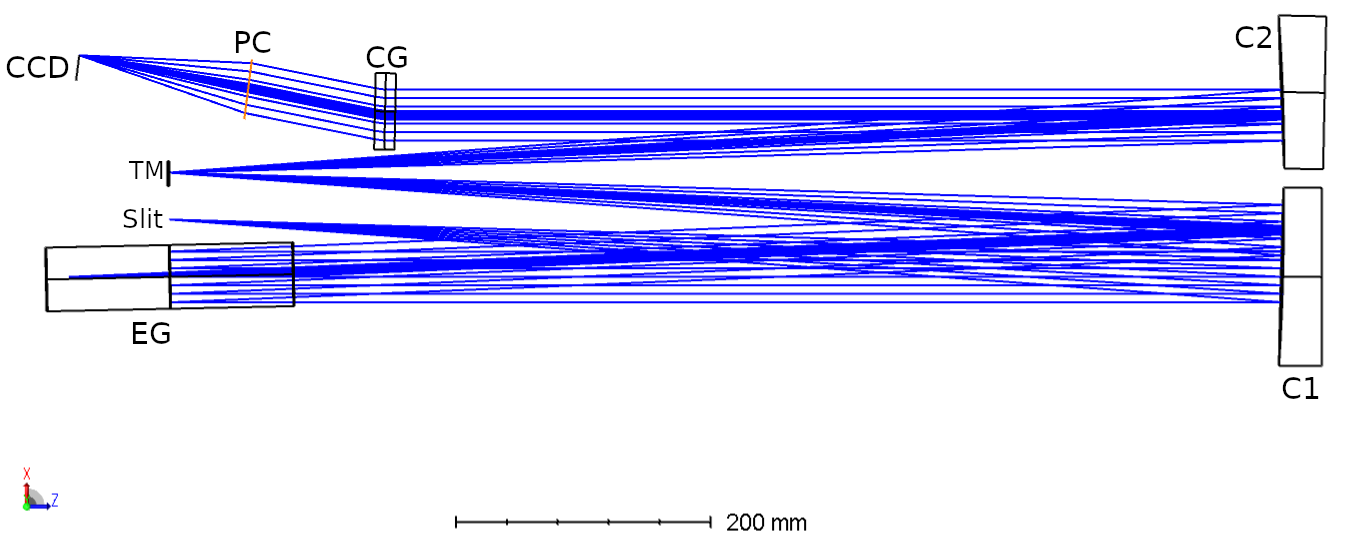
\includegraphics[width=\textwidth]{platospec_pre.png}
    \caption{Optical layout of PLATOSPEC spectrograph preliminary design.}
    \label{fig:ol}
\end{figure}

Table~\ref{tab:optical_data} show the main features of the optical design used to compute the ray tracing simulations. Fig.~\ref{fig:echellogram} show the echellogram for a detector array of 2048$\times$2048 pixels with 13.5$\mu$m pixel size computed by $\texttt{moes}$.

\begin{table}[h!]
    \centering
    \begin{tabular}{|c|c|}
    \hline
    Slit & D = 100$\mu$m \\
    Collimator & $f_{col}$ = 876~mm \\
    Main dispersion & Echelle grating, 41.6~lines/mm, 76$^\circ$ blaze angle\\
    Cross-dispersion & Transmission grating, 340~lines/mm\\
    Camera & $f_{cam}$ = 240~mm \\
    Detector size & 27.6~mm$\times$27.6~mm \\
    \hline
    \end{tabular}
    \caption{Caption}
    \label{tab:optical_data}
\end{table}

\begin{figure}[h!]
    \centering
    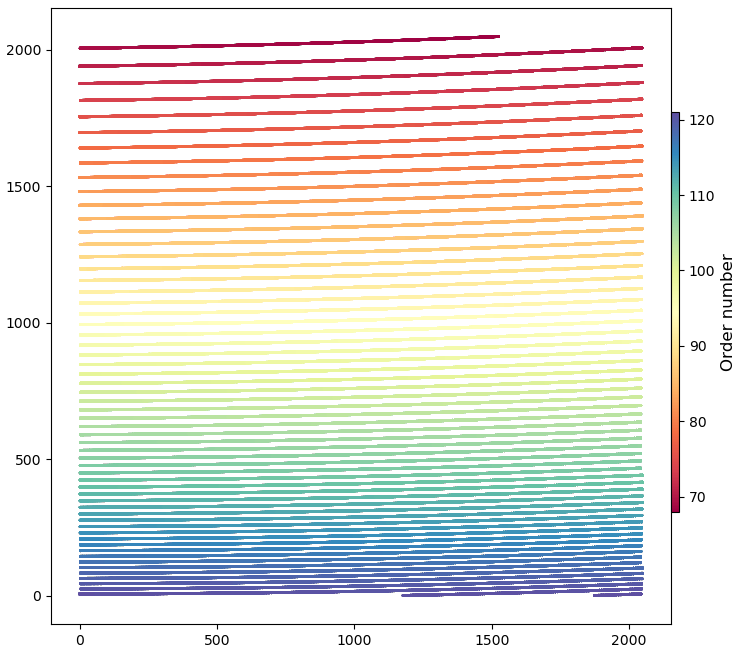
\includegraphics[width=0.75\textwidth]{echellogram_platospec.png}
    \caption{PLATOSPEC echellogram for a detector array of 2048$\times$2048 pixels with 13.5$\mu$m pixel size.}
    \label{fig:echellogram}
\end{figure}
Fig.~\ref{fig:template} show a portion of the stellar template used to create the observed RV shifted stellar spectra. The $\texttt{moes}$ software receives as an input the spectral order, the wavelengths and fluxes from the stellar template and the initial position of the slit. The output is the $(x,~y)_{CCD}$ coordinate of each spectral feature on the detector plane.

To create a 1D spectrum from our model we average the value of the fluxes within each pixel to obtain a 1D spectrum for each spectral order, with a length given by the number of pixels of the detector modeled.

\begin{figure}[h!]
    \centering
    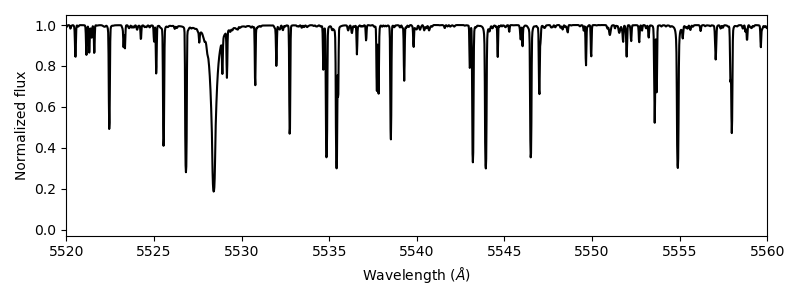
\includegraphics[width=0.8\textwidth]{template_spec.png}
    \caption{Normalized synthetic spectrum of a typical G-type star. This spectrum is used as a template for the creation of the $\texttt{moes}$ spectra observations.}
    \label{fig:template}
\end{figure}

\begin{figure}
    \centering
    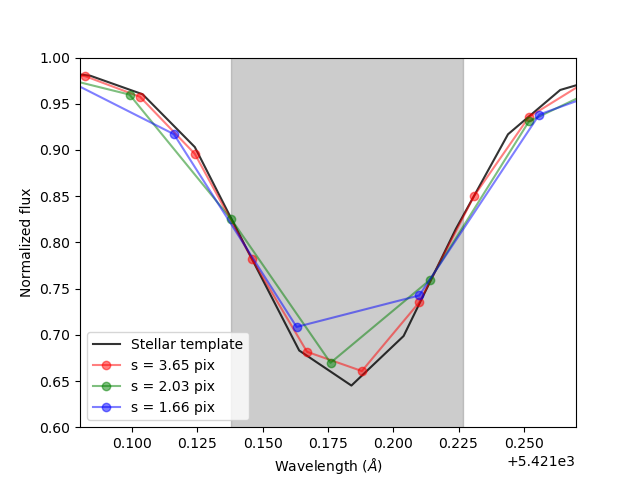
\includegraphics[width=0.5\textwidth]{line_example_mask.png}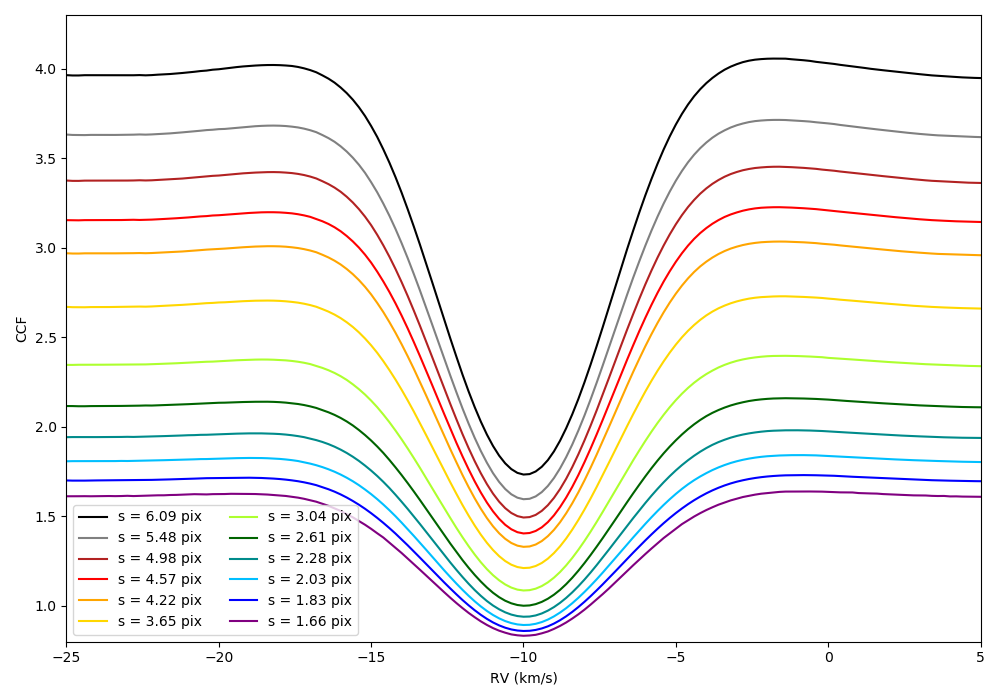
\includegraphics[width=0.5\textwidth]{ccf_compare.png}
    \caption{\textit{Left}: Close-up of a spectral line of the stellar template (black) modeled by \texttt{moes} at different spectral samplings $s$. The gray area shows the wavelength range covered by a typical binary mask of a G-type star. \textit{Right}: CCF for a nominal RV shift of -10\,000~m/s color coded by spectral sampling.}
    \label{fig:mask}
\end{figure}
Figure \ref{fig:mask} show a typical spectral line used in the computation of the CCF. The gray area show the wavelength range covered by the binary mask associated to that particular line. The black line corresponds to the stellar template, while the red, green and blue lines correspond to \texttt{moes} simulated spectra at sampling of 3.65, 2.03 and 1.66, respectively. One can clearly observe that the number of  pixels that fall within the wavelength range of the binary mask decrease as the spectral sampling decreases.


\section{Results and Analysis}
The grid of RV shifts ranges from -10000~m/s to 10000~m/s with steps of 50~m/s providing a total of 400 simulated observations for each of the detectors modeled. Figure~\ref{fig:mask} show the CCF calculated in spectra with a \textit{nominal RV} shift of -10000~m/s color-coded by the average spectral sampling. It shows the strong effect of spectra pixelization over the shape of the CCF. The larger the sampling the stepper and less broadened is the CCF. This is explained by the fact that decreasing the spectral sampling will decrease also the number of pixels that fall within the binary mask used to compute the CCF, having a direct impact over its shape. 

We use a $\chi^2$ minimization routine to fit a gaussian function to the CCF. The mean of the best gaussian fit corresponds to the \textit{measured RV}. Therefore, as an estimate of the accuracy of the instrument we have defined the quantity $\Delta RV$ as the difference between the \textit{nominal RV} and the \textit{measured RV}. 
This can be written as 
\begin{equation}
    \Delta RV = RV_{nom} - RV_{CCF}
\end{equation}
where $RV_{nom}$ correspond to the nominal RV shift of the simulated spectra and $RV_{CCF}$ corresponds to the RV measured in the simulated spectra using the CCF. %Therefore, for each one of the 400 spectra simulated, and for each of the detectors considered, we obtain a value for $\Delta RV$.

\begin{figure}
    \centering
    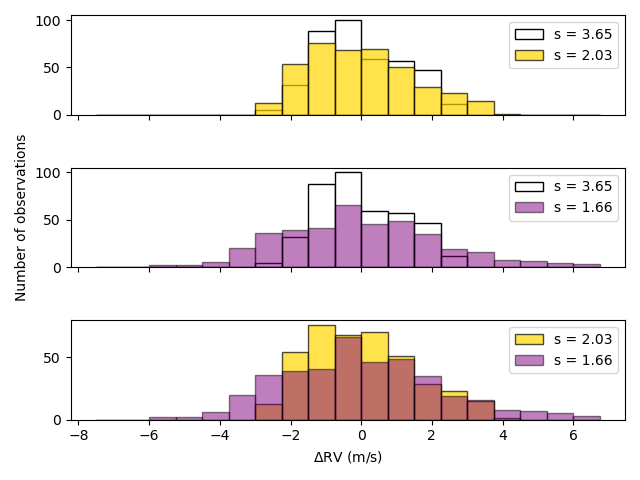
\includegraphics[width=0.455\textwidth]{sampling_vs_accuracy.png}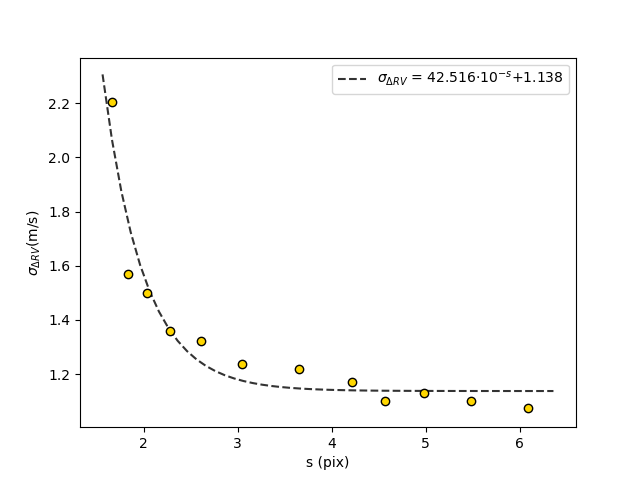
\includegraphics[width=0.5\textwidth]{sampling_vs_rvdiff.png}
    \caption{\textbf{Left}: \textit{Top panel}: Distribution of $\Delta RV$ values for $s = 3.65$ and $s = 2.03$. \textit{Central panel}: Distribution of $\Delta RV$ values for $s = 3.65$ and $s = 1.66$. \textit{Bottom panel}: Distribution of $\Delta RV$ values for $s = 2.03$ and $s = 1.66$. \textbf{Right}: RV accuracy $\sigma_{\Delta RV}$ as a function of spectral sampling for PLATOSPEC considering a detector size of 27.6~mm$\times$27.6
    mm.}
    \label{fig:drv_histo}
\end{figure}

Figure~\ref{fig:drv_histo} show the distribution of $\Delta RV$ values for three different values of spectral sampling $s$, 3.65~pix, 2.02~pix and 1.66~pix. The widest distribution is the one with sampling s=1.66~pix. While the peak of the s=3.65~pix distribution is higher than the peak of the s=2.02 pix, the difference in their widths is not considerably pronounced. However, when we compare the s=3.65~pix and s=2.02~pix distributions with the one with s=1.66~pix, the latter is considerably wider. 

We have considered the standard deviation of the distribution of $\Delta RV$, $\sigma_{\Delta RV}$, as a quantitative measure of the RV accuracy of the instrument. Figure~\ref{fig:drv_histo} show $\sigma_{\Delta RV}$ as a function of spectral sampling $s$ and Table~\ref{tab:res} summarize the main results. We observe a dependancy between spectral sampling and RV accuracy for values of $s<3$, which becomes stronger as spectral sampling decreases.  The RV accuracy does not seem to improve for values of $s$ larger than 4.57~pix. For values of $s$ smaller than 4.57~pix, $\sigma_{\Delta RV}$ becomes systematically larger as $s$ decreases. We observe a big jump in the RV accuracy when we go from sampling 1.83~pix to 1.66~pix, as it increases from 1.569~m/s to 2.205~m/s.

Typically, when designing echelle spectrographs to measure precision stellar RV, the Nyquist Criterion is used as a general rule of thumb for optimizing the average spectral sampling to 2.6~pix. Many high precision doppler velocimeters have spectral samplings larger than this value, with some examples where the spectral sampling is about 2~pix (buscar referencia). In the case of PLATOSPEC we aim to use a 2k$\times$2k detector with 13.5~$\mu m$ pixel size. With this detector the expected RV accuracy would be of about 1.5~m/s according to our simulations. This value is smaller than the 4-5~m/s RV precision expected for PLATOSPEC. Hence, the CCD proposed for PLATOSPEC is suitable to measure RVs accurate enough to conduct exoplanet searches.

\begin{table}[h!]
    \centering
    \begin{tabular}{|c|c|c|c|c|}
    \hline
    \# & Pixel size ($\mu m$) & w~(pix)$\times$ h~(pix) & s~(pix) & $\sigma_{\Delta RV}$ (m/s) \\ \hline
    1 & 4.5 & 6144$\times$6144 & 6.09 & 1.074\\ 
    2 & 5.0 & 5530$\times$5530 & 5.48 & 1.102\\ 
    3 & 5.5 & 5027$\times$5027 & 4.98 & 1.129\\ 
    4 & 6.0 & 4608$\times$4608 & 4.57 & 1.099\\ 
    5 & 6.5 & 4254$\times$4254 & 4.22 & 1.169\\ 
    6 & 7.5 & 3687$\times$3687 & 3.65 & 1.221\\ 
    7 & 9.0 & 3072$\times$3072 & 3.04 & 1.237\\ 
    8 & 10.5 & 2634$\times$2634 & 2.61 & 1.321\\ 
    9 & 12.0 & 2304$\times$2304 & 2.28 & 1.361\\ 
    10 & 13.5 & 2048$\times$2048 & 2.03 & 1.501\\ 
    11 & 15.0 & 1844$\times$1844 & 1.83 & 1.569\\ 
    12 & 16.5 & 1676$\times$1676 & 1.66 & 2.205\\ \hline
    \end{tabular}
    \caption{}
    \label{tab:res}
\end{table}

 
\section{Conclusions}
The relation between pixelization and RV accuracy in echelle spectrographs was investigated using ray tracing simulations. These simulations provide an accurate description of the optical path of single rays through any type of optical system. In particular, we simulated the ray tracing through PLATOSPEC, an echelle spectrograph designed to measure stellar RVs with a precision of about 4-5~m/s. 
Our main goal was to study the effect of detector pixelization in the accuracy of the stellar RVs measured by the spectrograph. In this context, we used a ray tracing algorithm to create a grid of RV shifted simulated spectra of a stellar template of a G-type star. By comparing the nominal RV given to the spectra, with the RV measured on the simulated spectra using the CCF we have estimated the RV accuracy of the spectrograph for a set of squared detectors with a fixed size but different pixel size and, consequentially, number of pixels. 

The results obtained show that for samplings higher than about 4.5~pix the RV accuracy does not increase considerably. For samplings smaller than 4.5~pix, the RV accuracy decreases with a significant decrement for samplings lower than 1.8~pix. For a detector with 2048$\times$2048~pix and 13.5$\mu m$ pixel size the RV accuracy is about 1.5$\mu m$, which is smaller than the expected 4-5~m/s RV precision of PLATOSPEC. Therefore, the 2k$\times$2k detector is suitable for its use in the PLATOSPEC instrument to conduct exoplanet searches using the RV method.

\printbibliography
\end{document}